\documentclass[11pt]{article}
\setlength{\parindent}{0pt}
\setlength{\baselineskip}{12.65pt}


\usepackage{pdfpages}
\usepackage[utf8]{inputenc}
\usepackage{eurosym}
\usepackage{url}
\usepackage[margin=20mm]{geometry}

%\usepackage{fancyhdr}
%\pagestyle{fancy}

%
%Die eingegangenen Projektskizzen werden nach folgenden Kriterien bewertet:
%– Zielabdeckung: Das Vorhaben ist auf die Vermittlungsziele des Wissenschaftsjahres 2019 zugeschnitten (Berück-
%sichtigung der Handlungsfelder, Zielgruppen, Forschungsinhalte).
%– Fachliche Kompetenz: Der Antragsteller ist qualifiziert, das Vorhaben durchzuführen und verfügt über nachgewie-
%sene Expertise über das Themenfeld und/oder die Vermittlung des Themenfelds.
%– Schlüssigkeit und Konsistenz des Konzepts: Idee, Ziele, Budgetschätzung.
%– Kommunikative Ausrichtung und Wirksamkeit: Das Vorhaben wird von geeigneten Kommunikationsmaßnahmen be-
%gleitet, es ist öffentlichkeitswirksam und generiert voraussichtlich eine mediale Berichterstattung. Das Vorhaben wird
%kommunikativ in das Wissenschaftsjahr 2018 eingebunden und als Teil dessen wahrgenommen.
%– Innovation: Das Vorhaben ist innovativ und leistet einen Beitrag zur Weiterentwicklung der Wissenschaftskommuni-
%kation in Deutschland.
%– Überregionalität und Nachhaltigkeit: Das Vorhaben strahlt überregional aus und/oder kann übertragen bzw. nachgenutzt werden


\begin{document}


\begin{center}
%\vspace{-13cm}
{ \centering 
\includegraphics[width=10cm]{hsf.png} }

\vspace{-0.8cm}
\begin{figure*}[h!]
\centering
\includegraphics[width=0.6\textwidth]{images/hand.jpg}
\end{figure*}
%\vspace{-1.8cm}

{\Huge
PROJEKTSKIZZE: Lernen in Handarbeit
}
\\
\vspace{0.5cm}

\Large
{\bf Antragsteller:} Prof. Dr. Alexander Gepperth (HDR)\\
{\bf Adresse: } Fachbereich Angewandte Informatik der HAW Fulda\\
Leipzigerstr. 123, 36037 Fulda\\
{\bf Email: } alexander.gepperth@cs.hs-fulda.de\\
{\bf Telefon: } 0661 9640 3485\\
\vspace{0.5cm}
%
{\bf Projektdauer:} 9 Monate\\
%\vspace{0.5cm}
%
{\bf Gesamtkosten:} 52.000\euro\\
%\vspace{0.5cm}
%
{\bf Zuwendungsbedarf:} 52.000\euro\\
\vspace{0.5cm}

%{\bf Konsortium:} Assisted Living, Hilfe für Schwerbehinderte, Service-Robotik, 3D-Simulation
\end{center}
%\end{titlepage}
\newpage

\renewcommand{\thesection}{1}
\section{Ausgangsfrage und Ziele des geplanten Vorhabens}
%
\begin{figure}[t!]
\centering
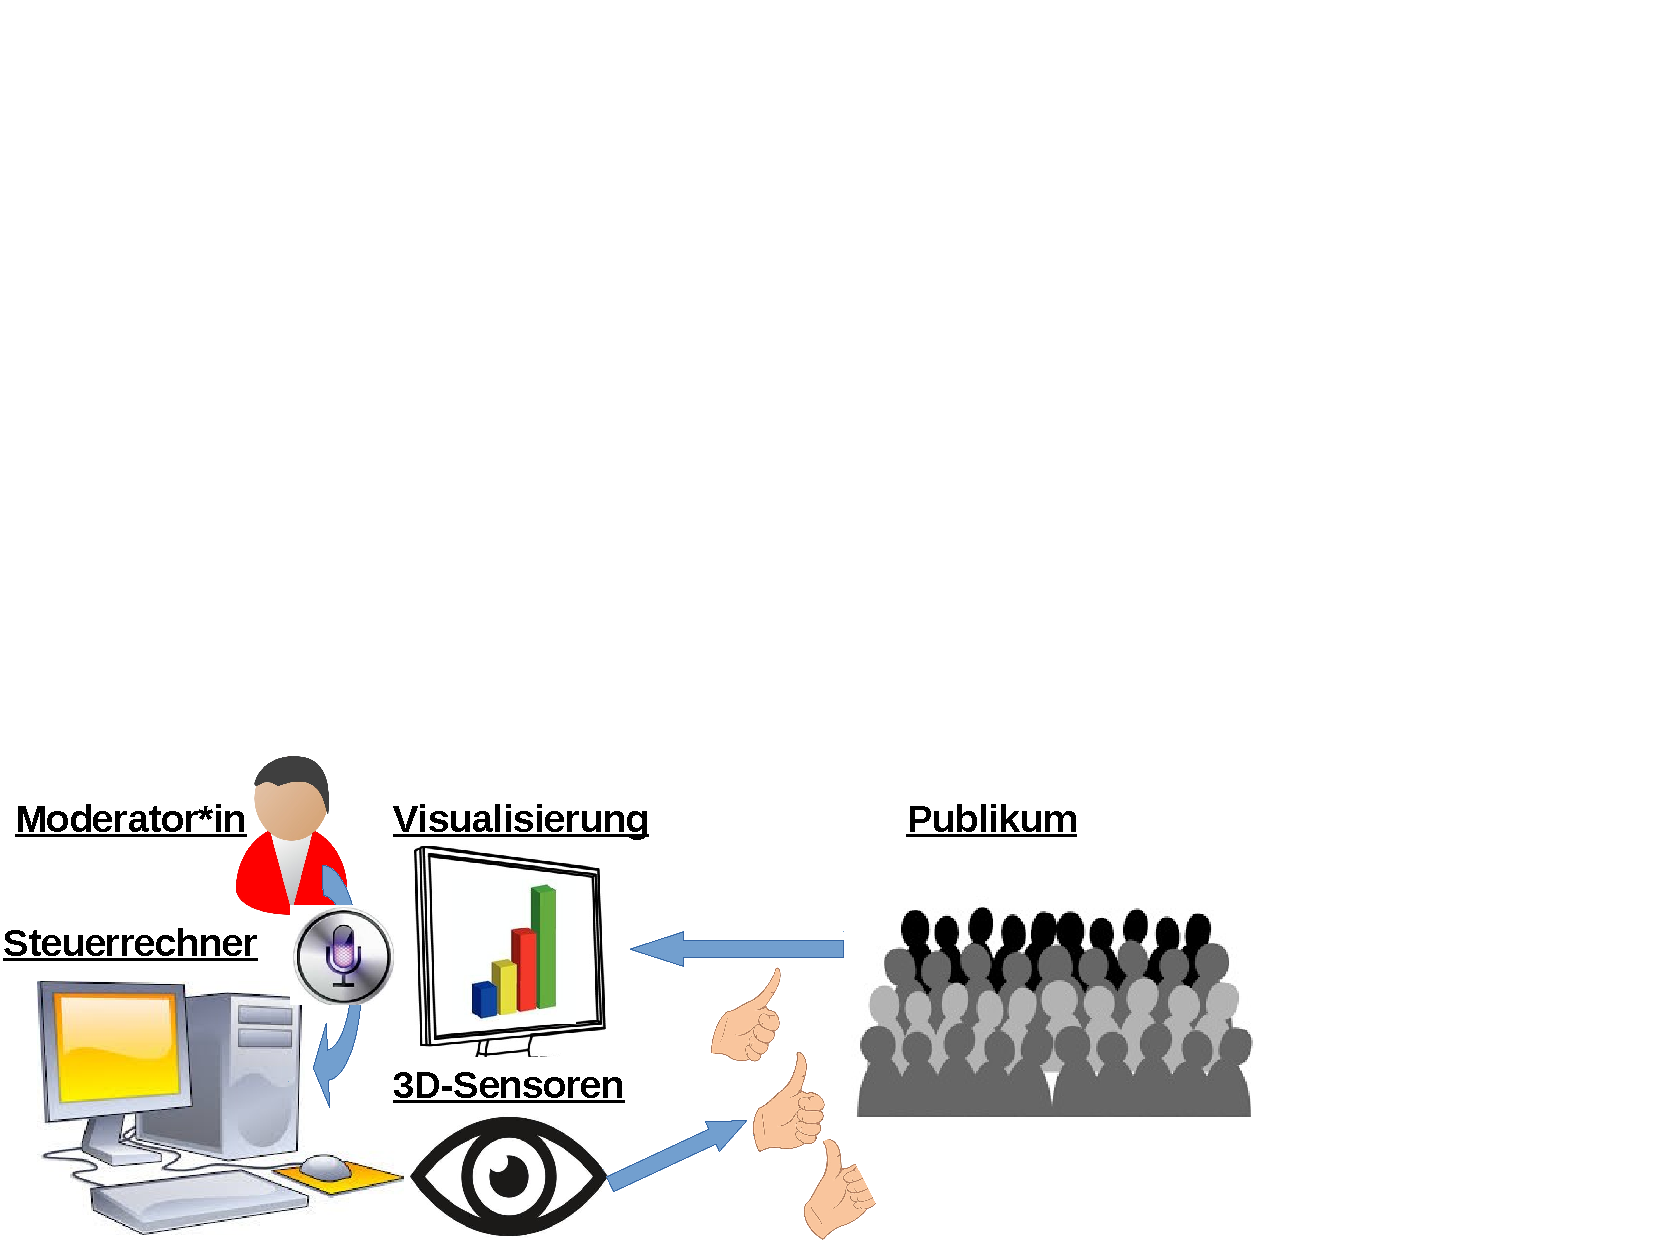
\includegraphics[viewport=0in 0in 7.8in 3.5in,width=0.7\textwidth,clip]{setup.pdf}
\caption{\label{fig:setup}
Schema des Formats, in dem der geplante Demonstrator für Handposen benutzt wird. Ein Steuerrechner, per Sprachsteuerung von einer Moderator*in kontrolliert, beobachtet mit einem oder mehreren 3D-Sensoren die Handgesten, die von multiplen Teilnehmer*innen aus dem Publikum durchgeführt werden. Die so gewonnenen Daten werden benutzt, um in Interaktion mit dem Publikum ein maschinelles Lernverfahren zu trainieren, welches dessen interner Zustand aufbereitet und auf eine für das Publikum leicht verständliche Art am Projektor visualisiert wird. Die Moderator*in kann bestimmte, besonders instruktive Situationen gezielt herstellen und erläutern.
}
\end{figure}
\subsection{Kurzzusammenfassung}
Das Projekt hat zum Ziel, ein interaktives Demonstrationssystem zur Veranschaulichung der Arbeitsweise maschinellen Lernens zu erstellen (siehe Abb. \ref{fig:setup}).
Gegenstand des Lernens sind Handposen, die dem integrierten maschinellen Lernverfahren interaktiv durch direkte Demonstration vermittelt werden, bzw. welche das System nach
erfolgter Demonstration erkennt.  Hierbei wird nach jeder Erkennung der interne Zustand des Lernverfahrens, welcher zu einer Entscheidung geführt hat, visualisiert.
Die hauptsächlichen Erkenntnisse zum maschinellen Lernen, die vermittelt werden sollen, lauten wie folgt: zunächst soll klargemacht werden, dass maschinelles Lernen alles andere als unfehlbar ist, vor allem dann, wenn Anzahl und Qualität der Daten unzureichend sind. Weiterhin soll durch eine detaillierte Visualisierung des internen Zustands des Lernverfahrens dargestellt werden, dass die grundsätzliche Arbeitsweise solcher Lernverfahren keine "schwarze Magie" darstellt, sondern auf anschaulicher Ebene  verstanden werden kann.
Zu guter Letzt soll mit den im Laufe der Demonstration trainierten Handposen eine Applikation oder ein Spiel gesteuert werden, um die Praxisrelevanz zu verdeutlichen und zu transportieren, dass maschinelles Lernen auch großes Potential für Unterhaltung und Amüsement bietet.
%
\subsection{Grundsätzliche Zielsetzung}
%
Maschinelles Lernen wird in er populären Wahrnehmung vielmals als mathematisch komplex und für Laien unverständlich wahrgenommen. Da maschinelle Lernverfahren in zunehmender Weise über Aspekte unseres täglichen Lebens entscheiden (z.B. bei der Kreditvergabe), führt diese Intransparenz nach unserer Auffassung dazu, das Misstrauen gegenüber maschinellen Lernverfahren zu erhöhen. Dem kann entgegengewirkt werden, indem gerade jungen Menschen vermittelt wird, dass
die grundsätzliche Funktionsweise solcher Verfahren einfach nachzuvollziehen ist, sowie dass die Fähigkeiten von Lernverfahren fast ausschließlich von den Daten abhängen, mit denen sie trainiert werden. Das Ziel soll sein, dass maschinelle Lernverfahren als das gesehen werden was sie sind: als Werkzeuge, deren Funktionsweise man verstehen kann, statt als intransparente Entscheider.
Das wird erreicht, indem Benutzergruppen in die Lage versetzt werden, ihr "eigenes" Lernverfahren durch direkte Demonstration zu trainieren, wobei live visualisiert wird, {\it warum} ein Verfahren zu einer bestimmten Entscheidung kommt.
%
%\newpage
\renewcommand{\thesection}{2}
\section{Ausführliche Vorhabensbeschreibung}\label{sec:besch}
\subsection{Einsatzszenario und Zielgruppen}\label{sec:zg}
%
An der HAW Fulda existieren vielfältige Formate des Austauschs mit lokalen Schulen und der interessierten Öffentlichkeit, welche im Rahmen des MINTMachclub: \footnote{\url {https://www.hs-fulda.de/kooperieren/schulen/mintmachclub-fulda/}} der Hochschule gebündelt werden: Kinder-Universität, MINT-Labortage, Girl's day, First LegoLeague sowie reguläre Besuche von Schulklassen, oft aus der gymnasialen Oberstufe zur Hinführung auf ein mögliches Studium. Für die interessierte Öffentlichkeit aller Altersstufen existieren die Formate Science-Slam und MINT-Kino. Auch existiert ein reger Austausch zwischen der Hochschule und weiter führenden Schulen des Landkreises, im Rahmen von Kollaborationen die Oberstufenschüler*innen die Teilnahme an Vorlesungen ermöglichen, aber auch durch offene Diskussionsrunden und Themenabende unter Teilnahme von Dozenten der Hochschule\footnote{z.B. am 24.11. 2017, siehe \url{http://www.winfriedschule-fulda.de/nachrichten-presse/nachrichten/archiv.html?}}. Genau diese Zielgruppe soll auch im Rahmen des vorgeschlagenen Projekts angesprochen werden. Sie besteht also aus jungen bis sehr jungen Menschen, und vor allem aus Schüler*innen. In dieser Zielgruppe herrscht großes Interesse gegenüber maschinellem Lernen (und generell gegenüber neuen Technologien), bei gleichzeitiger weitgehender Unkenntnis der Funktionsprinzipien.
Weiterhin wird diese Zielgruppe erfahrungsgemäß eher durch interaktive Formate angesprochen und begeistert, speziell in den niedrigeren Klassen.

Da das Projekt eine relativ heterogene Zielgruppe anspricht, vor allem im Bezug auf das Alter, ist es sicherlich sinnvoll, die Demonstration flexibel an das Publikum anzupassen, so dass die Kernideen auf jeden Fall transportiert werden können:
rein interaktiv und relativ kurz für Schüler*innen ohne Informatik-Erfahrung, oder beispielsweise programmierbar für Oberstufenklassen im Rahmen eines Vormittagsprojekts.
%
\subsection {Ablauf einer Demonstration}
%
\begin{figure}[t!]
\centering
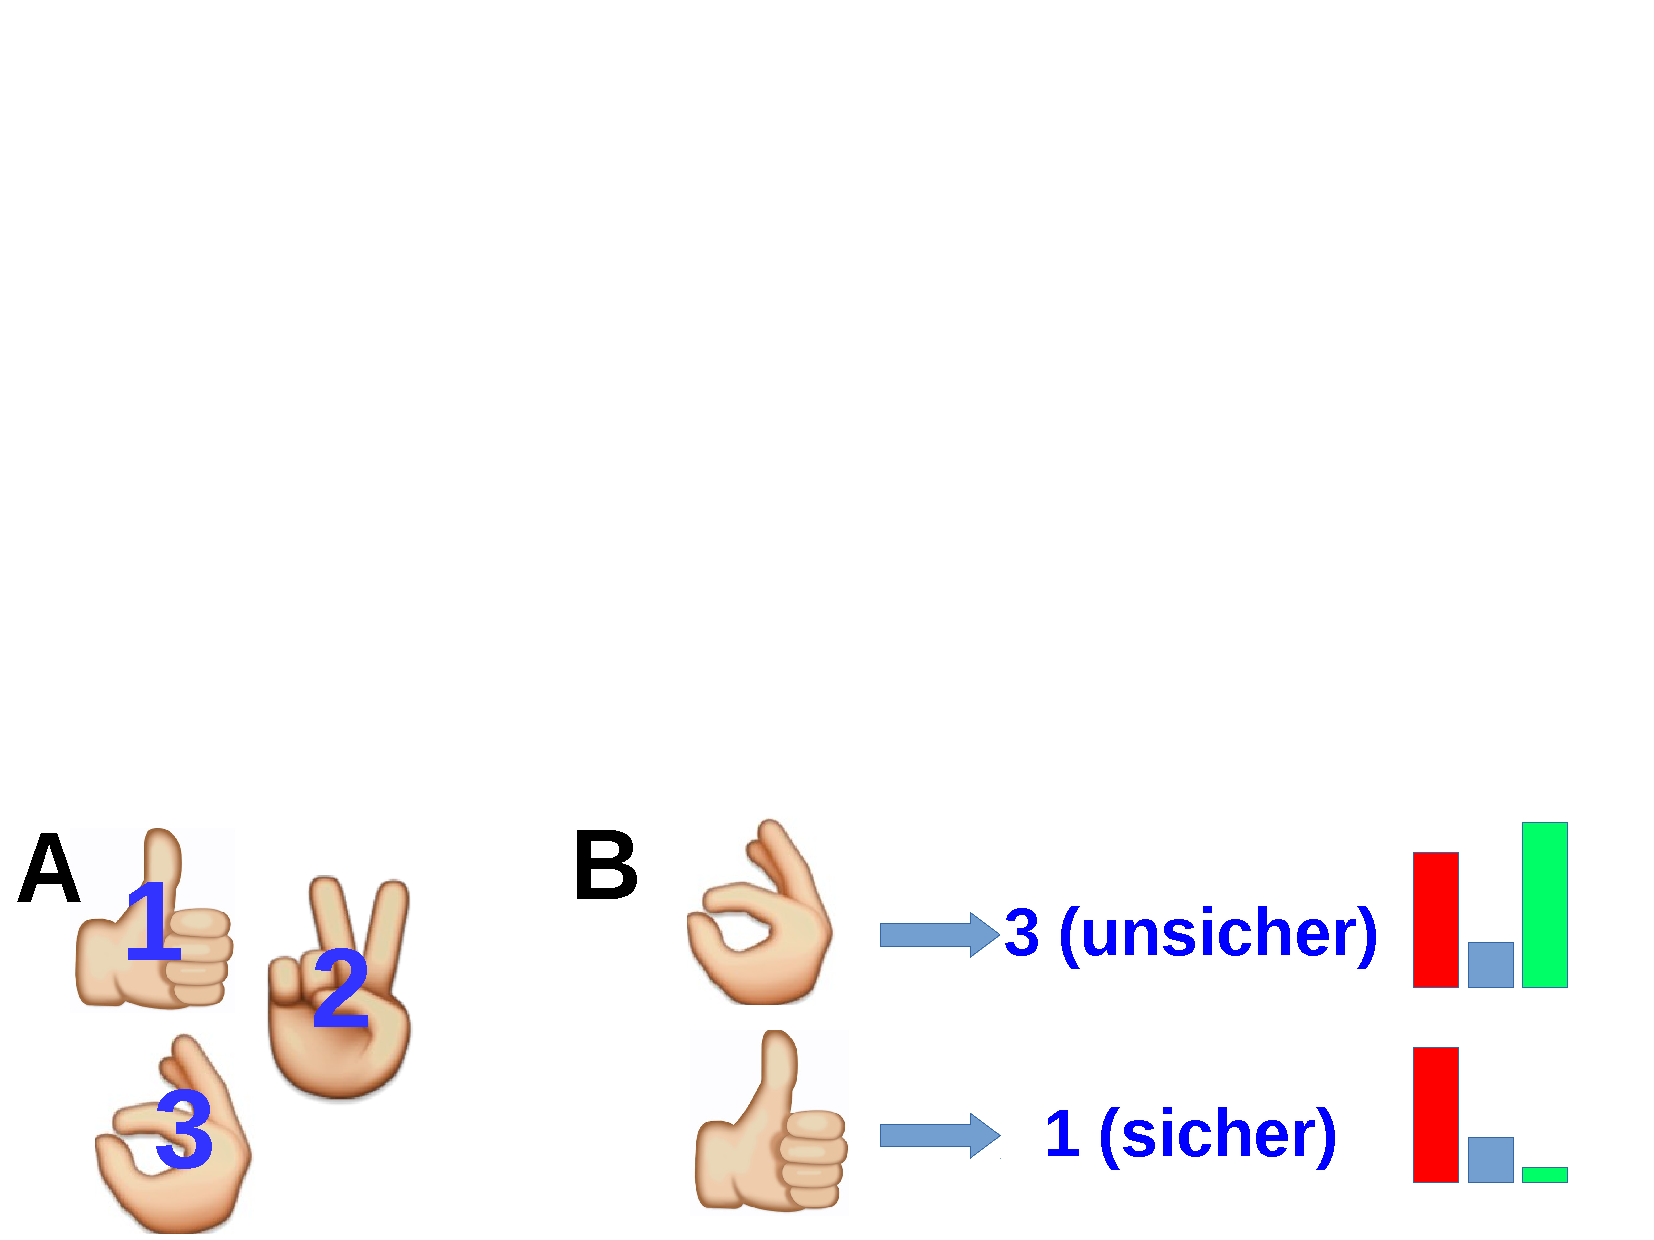
\includegraphics[viewport=0in 0in 11in 2.8in,width=0.7\textwidth,clip]{phases.pdf}
\caption{\label{fig:phases}
Übersicht über die drei Hauptphasen einer Demonstration (nicht gezeigt ist die letzte Phase, in der die trainierten Handposen für Unterhaltungszwecke genutzt werden. Links (A): Definition der Handposen (Phase 1) sowie Trainieren des Demonstrators durch das Publikum (Phase 2). Rechts (B): Tests des Demonstrators durch das Publikum: der Demonstrator zeigt jeweils die von ihm erkannte Handpose an, sowie zusätzlich eine Visualisierung seines internen Zustands, so dass die Entscheidung verstanden werden kann (schematisch eingezeichnet, tatsächliche Visualisierung wird abweichen).
}
\end{figure}
%
Als Zielgruppe einer Demonstration wird eine Gruppe von mindestens 10 Personen und maximal 30 Personen angenommen, was sicherstellt, dass eine Schulklasse komplett daran teilnehmen kann.
Eine Demonstration besteht aus drei Hauptphasen, siehe Abb. \ref{fig:phases}.
Die erste Demonstrationsphase besteht aus der gemeinsamen Definition der zu benutzenden Handposen.
In der zweiten Phase demonstrieren bis zu 10 Personen gleichzeitig, auf Aufforderung des Demonstrators, einzelne Handposen, welche von Demonstrator registriert und zum Training des internen maschinellen Lernverfahrens genutzt werden.
In der folgenden dritten Phase demonstrieren einzelne Personen, auf Aufforderung des Demonstrators, mehrere der zuvor vereinbarten und dem Demonstrator antrainierten Handposen. Für jede dieser Posen gibt der Demonstrator seine Einordnungen (Klassifikationen) aus, wobei
ausführlich visualisiert wird, wie jede Klassifikation zustande gekommen ist (z.B. durch Anzeige der Einzelkonfidenzen und der Gesamtkonfidenz). Phasen 2 und 3 können beliebig oft wiederholt und der Lernfortschritt verglichen werden. Durch die Wiederherstellung vergangener Zustände und systematische Manipulation der gezeigten Handposen können verschiedene typische Effekte für fortgeschrittene Zielgruppen gezielt demonstriert werden, vor allem Overfitting und Generalisierung.

Als letzte Demonstrationsphase sollen die Teilnehmer die dem System antrainierten Handposen nutzen, um eine Anwendung zu kontrollieren, wobei sich
die Steuerung eines Spiels bzw die Steuerung eines autonomen Roboters anbieten. Auch eine zur Verfügung Stellung der erkannten Handposen per ReST API ist einfach umsetzbar,
wobei dann die Reaktion eines Computersystems auf eine bestimmte Handpose von fortgeschrittenen Teilnehmern im Rahmen einer Projektarbeitsphase selbst programmiert werden kann.
%
% TODO lernen der einschränkungen: linek hand trainieren, rechte testen --> problem!
\subsection{Technische Bausteine der Demonstration}
%
Für die Umsetzung des Demonstrators wird auf Techniken zurückgegriffen, welche bereits im Rahmen mehrerer Publikationen im Rahmen der Handposen- und Handgestenerkennung implementiert und erprobt wurden, siehe Kap. \ref{sec:eigen}. Hierbei ist im Besonderen die Verarbeitung von 3D-Sensordaten, deren Transformation in kompakte aber aussagekräftige Beschreibungen (Deskriptoren) sowie die praxisorientierte Anwendung maschineller Lernverfahren, insbesondere neuronale Netze und DNNs. Die Implementierung kann auf einem einzelnen, allerdings leistungsfähigen Rechner mit High-End Grafikkarte stattfinden, so dass sowohl die Sensordatenakquisition als auch deren Transformation in Deskriptoren sowie die Ausführung neuronaler Klassifikatoren mindestens 5 mal pro Sekunde erfolgen kann, idealerweise öfter. Die Steuerung und Konfiguration der einzelnen Phasen des Demonstrators soll durch ein einfaches Sprachinterface erfolgen.
%
\subsection{Popularisierung und Kommunikationsstrategie}
Um das Projekt einer breiteren Öffentlichkeit bekannt zu machen, soll zunächst Information über den Demonstrator auf der Web-Präsenz des MINTMachclubs der HAW Fulda (siehe \ref{sec:zg}) bereitgestellt werden. Einerseits soll der Demonstrator im Rahmen regelmäßig stattfindender Formate des MINTMachclubs zum Einsatz kommen, andererseits sollen die existierenden Kommunikationskanäle zu Schulen aktiv genutzt werden, um zu Besuchen an die HAW Fulda einzuladen oder ihn auch vor Ort in Schulen einzusetzen, wobei jeder Schulbesuch medial begleitet werden sollte, um größtmögliche Aufmerksamkeit zu generieren.
%
\renewcommand{\thesection}{3}
\section{Darstellung des Eigenanteils}\label{sec:eigen}
%
\begin{figure}[ht]
  \centering
  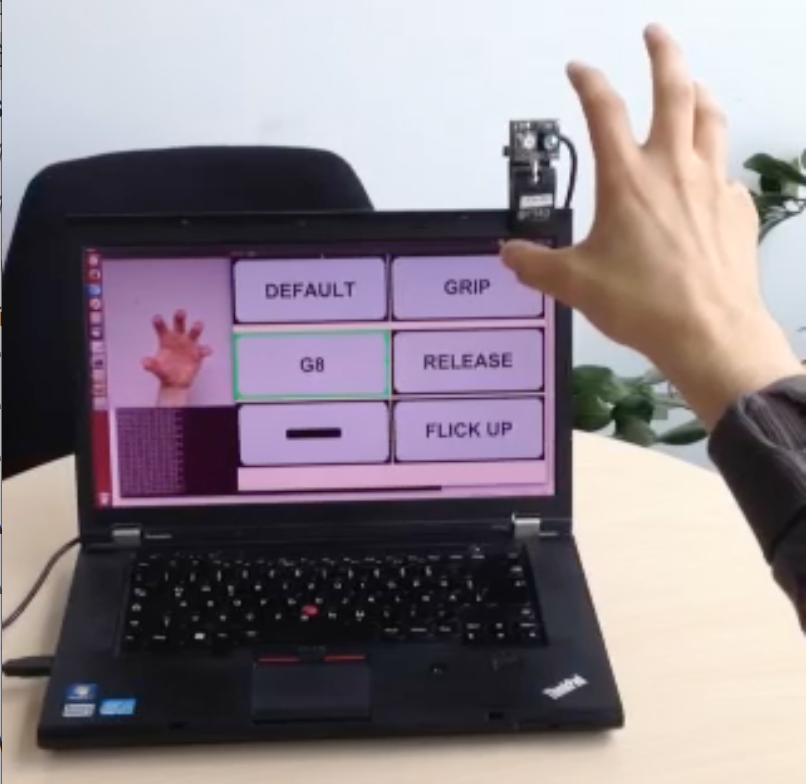
\includegraphics[width=0.4\textwidth]{images/s1.png}
  \caption{Im Rahmen eines früheren Forschungsprojekt implementierter Demonstrator zur Erkennung dynamischer Handgesten.}
  \label{fig:demo}
\end{figure}
%
\textbf{Eigenanteil, fachliche Befähigung} Der Antragsteller hat weit reichende Kompetenzen im Bereich des maschinellen Lernens mit neuronalen Netzen und Deep-Learning-Verfahren \cite{gepperth2018a,gepperth2018c,gepperth2017b}, sowie moderner Interaktionstechniken in Form von statischen Handposen und dynamischen Handgesten \cite{gepperth2017d,kopinski2016x3}. Im Bereich der modernen Interaktionstechniken (insb. dynamische Freihandgesten) wurde in bilateralen Forschungsvorhaben bereits ein Demonstrator zur Erkennung von Handgesten mittels 3D-Sensorik entwickelt, welcher hier mit geringfügigen Änderungen wieder zum Einsatz kommen soll (siehe Abb. \ref{fig:demo}). Mit Hilfe dieses Demonstrators konnten zahlreiche Erkenntnisse im Bereich des überwachten Lernens, der Sensordatenfusion und der Messung der kognitiven Last im Straßenverkehr gewonnen werden. So wurde in einem kooperativen Forschungsvorhaben nachgewiesen, dass die tatsächliche Ablenkung im Straßenverkehr während der Benutzung von Freihandgesten zur Steuerung von Infotainmentsystemen geringer ist als während der Bedienung durch Touchgesten oder Verwendung analoger Schaltelemente \cite{kopinski2016touch}.
%
\begin{figure}[ht]
  \centering
  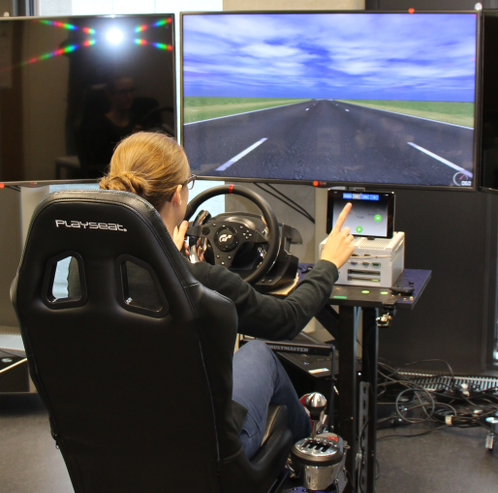
\includegraphics[width=0.4\textwidth]{images/simulator.png}
  \caption{Simulator}
  \label{fig1}
\end{figure}
%
Hierfür wurde der Demonstrator mit einem Straßenverkehrssimulator gekoppelt, und es konnten realistische Test mittels genormter Messanalysen durchgeführt werden. Aufbauend auf dem Demonstrator wurden darüber hinaus zahlreiche Forschungsergebnisse im Bereich der 3D Sensordatenfusion und der mehrstufigen Klassifikation erzielt und veröffentlicht. So waren grundlegende Erkenntnisse, dass Daten aus Time-of-Flight Kameras sowohl früh als auch spät fusionieren um eine Verbesserung der Erkennungsrate zu erzielen \cite{kopinskineural}. Dieses ist insbesondere dahingehend interessant, da es unterschiedliche Performancegewinne des Systems nach sich zieht, was insbesondere für Handgestenerkennung in Echtzeit von hoher Praxisrelevanz ist. Darüber hinaus wurde mit Hilfe von mehrstufigen neuronalen Netzen nachgewiesen, dass man Informationen aus bereits trainierten Netzen verwenden kann, um eine verbesserte Gesamtperformance des Systems zu erreichen, indem man die Erkennungsgüte mit vortrainierten Netzen stabilisiert \cite{kopinski2015pragmatic}. Diese Erkenntnisse bildeten die Grundlage für die Erkennung von Handposen und die Erkennung von dynamischen Handgesten auf Basis stabiler Posen \cite{kopinski2015real}. Letztlich wurde durch den Einsatz von Deep-Learning Verfahren ein eigener Ansatz entwickelt, mittels dessen Erkenntnisse aus dem Bereich der 2D-Bilderkennung in den 3D-Raum übertragen werden konnten \cite{kopinski2016x3,gepperth2017d}.\\

\textbf {Eigeninteresse} Die Erstellung des in Kap. \ref{sec:besch} dargelegten Simulators baut auf bereits implementierten und getesteten Demonstrationssystemen auf und verspricht daher, relativ zeiteffizient zu sein. Ein neuer Aspekt ist die Gewinnung von Trainingsdaten von mehreren Personen gleichzeitig: dies ist zwar konzeptuell unkritisch, erfordert aber signifikanten Arbeitsaufwand zur robusten Implementierung, weswegen seitens des Antragstellers ein starkes Interesse an Unterstützung bei der Umsetzung dieses Konzepts besteht. Ein solcher optimierter Demonstrator ist als Plattform für zukünftige Forschungs- und Lehraktivitäten sehr wertvoll. Dies wird in größerer Ausführlichkeit in Kap. \ref{sec:ueber} dargelegt. Abgesehen vom Eigeninteresse des Antragstellers ist auch das Interesse der Hochschule nicht zu vernachlässigen: die HAW Fulda ist auf einen steten Zustrom leistungsfähiger und motivierter Studierender angewiesen, vor allem auch aufgrund des neu verliehenen Promotionsrecht im Bereich Informatik. Gleichzeitig aber steht die Hochschule in einem harten Konkurrenzkampf um diese Zielgruppe mit benachbarten Hochschulen, Universitäten und auch Industrieunternehmen. Durch eine frühe Motivation junger Menschen für technische Fragestellungen, und durch die gleichzeitige Darstellung der eigenen Technologiekompetenz kann die HAW Fulda potentiell viele junge Menschen für ein Hochschulstudium vor Ort begeistern.
%
\renewcommand{\thesection}{4}
\section{Nachhaltigkeit,Übertragbarkeit}\label{sec:ueber}
\textbf {Forschungsprojekte} Der Antragsteller hat umfangreiche Vorarbeiten im Bereich des maschinellen Lernens erbracht, vor allem im Bereich der Handposen- und Gesten\-er\-kenn\-ung, der Objekterkennung sowie des inkrementellen Lernens mit neuronalen Netzen (DNNs), siehe Kap. \ref{sec:eigen}.
Ein implementierter Demonstrator so wie er in Kap. \ref{sec:besch} beschreiben ist, könnte für weiter gehende Forschungsprojekte und Forschungsanträge des Antragstellers von großem Nutzen sein, hauptsächlich aufgrund der Fähigkeit, Hand\-posen und Hand\-gesten von mehreren Personen gleichzeitig aufzunehmen. Dies kann die Akquisition eine großen Menge qualitativ hochwertiger Trainingsdaten, deren Gewinnung ja stets das Hauptproblem eines jeden Projekts im Bereich des maschinellen Lernens darstellt, stark vereinfachen. Des Weiteren kann der Demonstrator auch dazu dienen, methodische Fortschritte einfach zu verdeutlichen (z.B. als zusätzliche Ressourcen beim Einreichen eines Konferenzbeitrags oder als Live-Demo während eines Vortrags). Hierbei ist im Besonderen an die Arbeiten des Antragstellers zum inkrementellen Lernen zu denken, welche untersuchen, wie DNNs neue Kenntnisse dazulernen können \cite{gepperth2017b,gepperth2018a,gepperth2016tut,gepperth2015bio}. Anhand des Demonstrators lässt sich die Tatsache, dass ein Lernverfahren eine neue, soeben demonstrierte Handpose erfolgreich dazugelernt und die bereits vorher beherrschten nicht vergessen hat, lässt sich einfach und anschaulich demonstrieren.\\

\textbf{Lehre}
Der Antragsteller ist Modulverantwortlicher für die Module "Künstliche Intelligenz" und "Machine Learning" auf Bachelor-bzw. Master-Niveau. Vor allem auf Bachelor-Niveau wo die mathematischen Grundlagen des maschinellen Lernens noch nicht vertieft eingeführt werden können, wird es ein Demonstrator für Handposenerkennung ermöglichen, auch konzeptuell abstrakte Ideen wie z.B. Overfitting, Underfitting, Sampling Bias oder Generalisierung anschaulich zu erläutern. Selbstverständlich können auch die vom Demonstrator aufgenommenen Daten auch für kleine Projekte im Rahmen der Lehrveranstaltungen eingesetzt werden. Auch ein Einsatz im Bereich der Vorlesung "Robotik" ist sinnvoll, in welcher evtl. eine Handposensteuerung für autonome Roboter als Projekte umgesetzt werden kann.\\

\textbf{Wissenschaftliche Nachwuchsförderung} Im Rahmen des Promotionsrechts, welcher der HAW Fulda vor kurzem für das Fach Informatik verliehen wurde, ist die Gewinnung geeigneten wissenschaftlichen Nachwuchses sehr wichtig. Durch einjährige Mitarbeit an einem solchen Projekt können Studierende mit hohem Potential an die wissenschaftliche Arbeitsweise herangeführt und mit den notwendigen Techniken vertraut gemacht werden, um im Anschluss eine Promotion durchzuführen.\\

Zusammenfassend kann festgestellt werden, dass aufgrund des hohen Potentials des hier beschriebenen Demonstrators in Forschung und akademischer Lehre sichergestellt ist, dass ein solches System über viele Jahre hinweg im Einsatz bleiben wird, und somit der Einsatz der Projektmittel eine nachhaltige und langfristige Wirkung erzielt.
%

\newpage
\renewcommand{\thesection}{5}
\section{Finanzierungsplan}
Es werden die folgenden Kostenpunkte zur Durchführung de Projekts angesetzt. Jeder Punkt wird einzeln im Hinblick auf seine Notwendigkeit und Verhältnismäßigkeit
diskutiert und begründet. Generell wird davon ausgegangen, dass 4 Demonstratoren gleichzeitig ausgerüstet werfen, um bei "parallelen" Veranstaltungen jeder Gruppe eine Demonstration zeigen zu können. Dies ist bei Projekten, wo viele Schüler an einem oder zwei Tagen ein Projektprogramm absolvieren, relativ häufig der Fall und begründet diese Grundsatzentscheidung.
\begin{itemize}
%50\% Stelle Data Science E11 - TVL 11: 27.058,19
\item \textbf{1 Wissenschaftliche Mitarbeiter*in E11 - TVL 11/2 (27.058,19\euro)} Diese Mitarbeiter*in soll die Demonstrator-Plattform unter Anleitung des Antragstellers und unter Einbeziehung bereits existierenden Programmcodes implementieren. Gesucht wird eine Person mit stark ausgeprägten Programmierfähigkeiten und Erfahrung in der Sensordatenverbeitung. Da
zur Implementierung des Demonstrator-Plattform hauptsächlich bereits beschriebene Systeme umgesetzt werden sollen, sind außer Grundkenntnissen keine speziellen Kenntnisse des maschinellen Lernens nötig, was die Suche nach geeigneten Kandidaten deutlich erleichtern sollte.
\item \textbf{Sensoren: (2000\euro)} Hier ist die Beschaffung von ca. 6-8 3D-Sensoren (2 für jeden der 4 Demonstratoren) geplant. Diese Sensoren sollten bei Sonneneinstrahlung robust funktionieren, was reine Structured-Light-Ansätze ausschließt. Deshalb sind Hybridlösungen (Stereo + Structured Light) empfehlenswert, wie sie gegenwärtig für ca. 200\euro/Stück verfügbar sind.
\item \textbf{Rechner (10000\euro)} Es werden 4 möglichst identische Rechner plus ein Arbeitsplatzrechner für die Mitarbeiten*in benötigt. Deren Ausstattung muss ausreichend Speicher sowie ein starkes Netzteil umfassen, um eine leistungsfähige Grafikkarte zu versorgen, die für das Training und die effiziente Ausführung der maschinellen Lernverfahren unabdingbar ist.
\item \textbf{Deputatsermäßigung Antragsteller (2SWS, 1 Jahr, 2800\euro)} Dies ist erforderlich, um in ausreichendem Maße an der Projektarbeit teilnehmen zu können, insbesondere um die Projektmitarbeiter*in anzuleiten.
\item \textbf{2 stud. Hilfskräfte (6 Monate, 10h/Woche, ca. 10000\euro)} Eine Hilfskraft wird benötigt, um funktionale Tests des Demonstrators und Bugfixing durchzuführen, sowie um Aspekte der Usability zu verifizieren. Eine weitere Hilfskraft wird benötigt, um eine Projektwebseite zu erstellen und kontinuierlich zu pflegen. Dies beinhaltet vor allem, Bilder und Videos bereits durchgeführter Demonstrationen einzustellen sowie die Ankündigung folgender Demonstrationen aktuell zu halten
\end{itemize}

Hiermit ergibt sich ein Gesamtförderbedarf von ca. 52.000\euro.

\newpage
\renewcommand{\thesection}{6}
\section{Zeit- und Arbeitsplan}
\begin{figure}
\centering
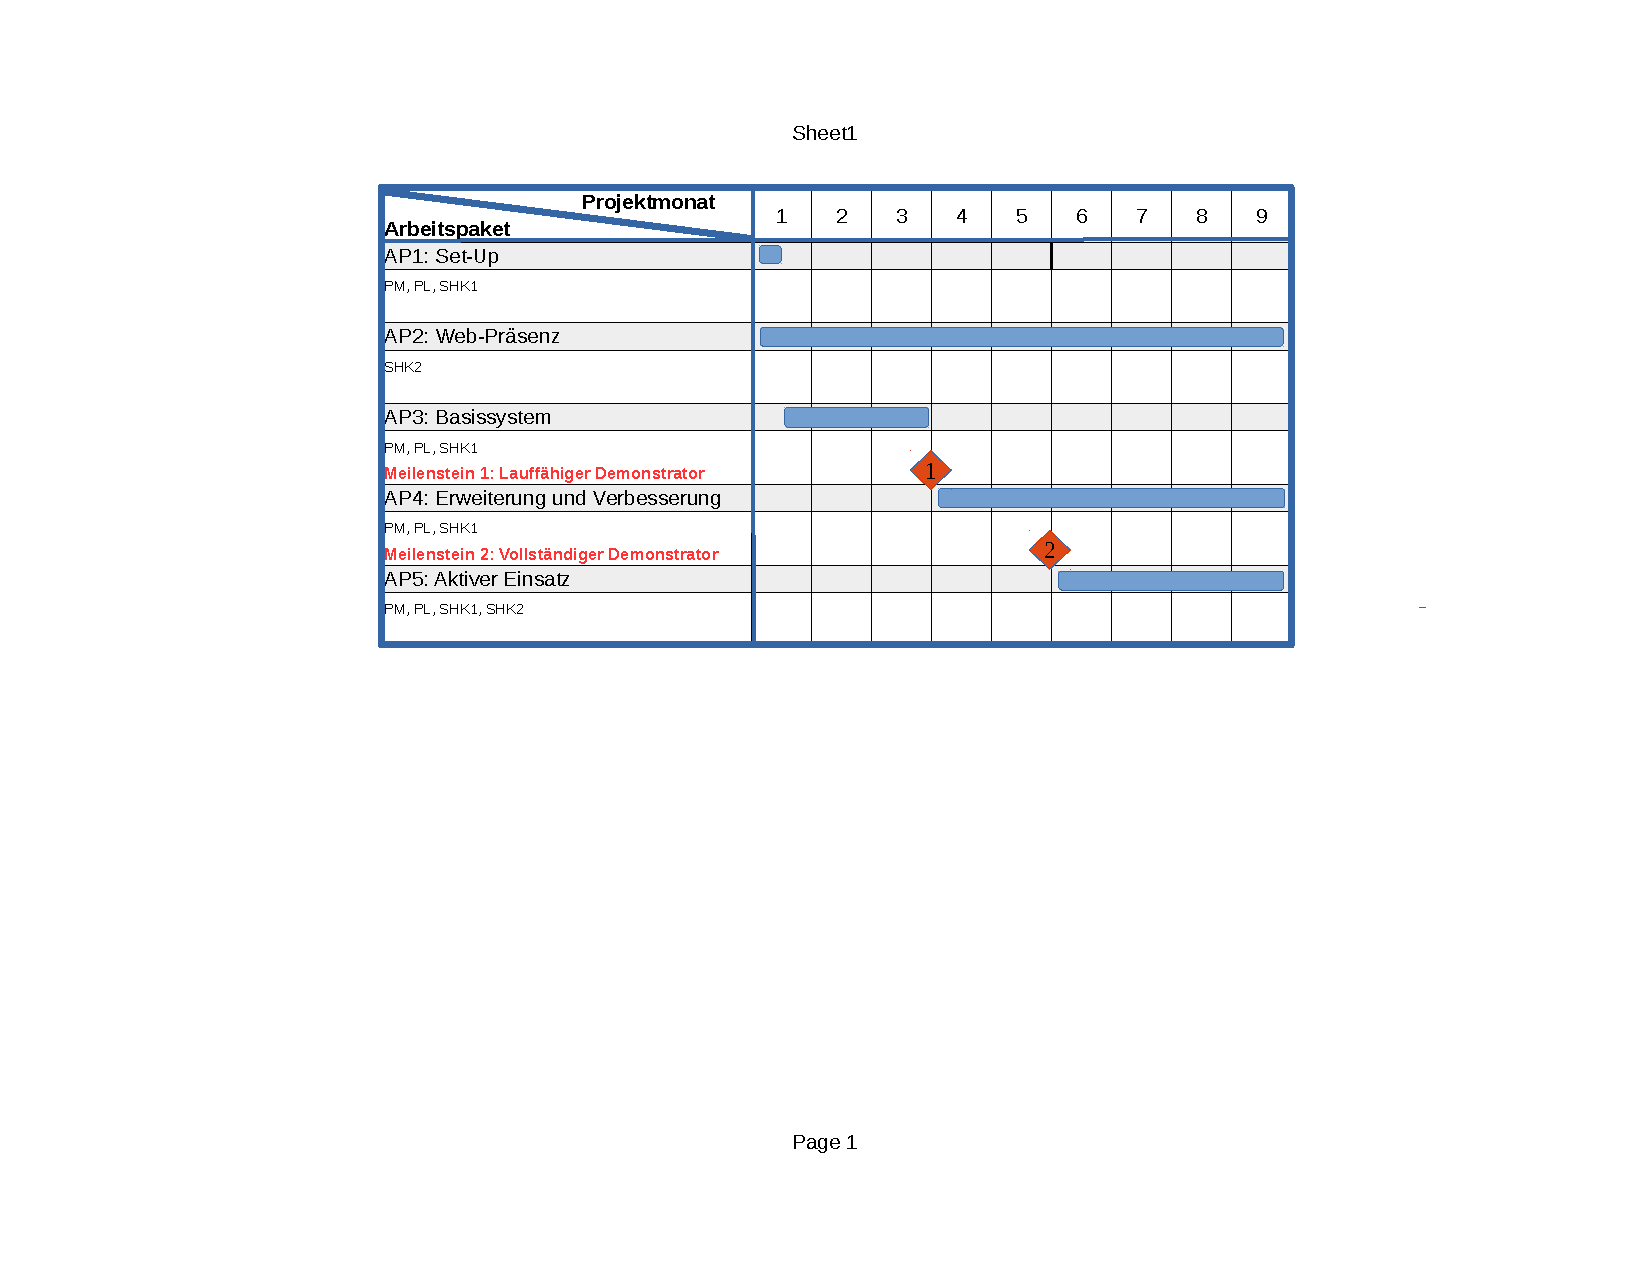
\includegraphics[viewport=2.5in 3.5in 8.8in 7.5in,width=0.7\textwidth,clip]{gantt.pdf}
\caption{Grafische Darstellung des geplanten Projektablaufs. Unter jedem Arbeitspaket werden
die daran beteiligten Mitarbeiter*innen genannt (Abkürzungen siehe Text).
}
\end{figure}
Der geplante Ablauf des Projekts ist im oben stehenden Gantt-Diagramm festgehalten.
Es wird von einer Projektlaufzeit von 9 Monaten ausgegangen, sowie von 3 prinzipiellen
Projektteilnehmern (siehe vorheriges Kapitel): der Projektmitarbeiter*in (PM), dem Projektleiter (PL) sowie den studentischen Hilfskräften (SHK1 und SHK2). Es muss durch geeignete Planung sichergestellt werden, dass bereits früh im Projekt Demonstrationen durchgeführt werden können, weswegen das Hauptaugenmerk der ersten Projekthälfte darauf liegt, möglichst schnell eine erste Version des Demonstrators fertigzustellen, auch wenn die Funktionalität oder Usability noch nicht voll ausgebildet sind. Folgende Arbeitspakete (APs) sind vorgesehen:
\begin{itemize}
\item \textbf {AP1: Set-Up der Hard-und Software} In diesem Schritt werden die Rechner und konfiguriert, die Sensoren beschafft sowie die grundlegenden Software-Pakete und Treiber installiert. Es ist vorgesehen, mit die Bibliothek PCL (siehe \cite{pcl}) zur 3F-Verarbeitung sowie die Bibliothek TensorFlow\cite{tf} zur Implementierung maschineller Lernverfahren zu nutzen.
\item \textbf {AP2: Set-Up der Web-Präsenz} Eine einfache Web-Präsenz soll so schnell wie möglich auf den Seiten des MINTMachclubs der HAW Fulda aufgebaut werden und die Funktionsweise des geplanten Demonstrators möglichst anschaulich beschreiben.
\item \textbf {AP3: Implementierung eines Basissystems} Eine erste Version des Demonstrators soll so schnell wie möglich fertig gestellt werden. Aufgrund dieser Maßgabe können Elemente wie die Aufnahme von Handposen mehrerer Personen, sowie die Sprachsteuerung des Demonstrators, zunächst zurückgestellt werden.
\item\textbf{AP4: Stetige Erweiterung und Verbesserung des Basissystems}
In dem Maße, wie im Rahmen von Demonstrationen neue Erfahrungen gewonnen werden, sollen Sie in das Design des Demonstrators einfließen. Hierfür ist es erforderlich, proaktiv Werbung für das System zu machen und auch Schulbesuche durchzuführen.
\item\textbf{AP5: Aktiver Einsatz und Dissemination}
Sobald der Demonstrator die in Kap. \ref{sec:besch} beschriebene Form erreicht hat, sollen die Bemühungen, ihn zu nutzen, durch verstärkte Öffentlichkeitsarbeit intensiviert werden.
\end{itemize}
%
%\renewcommand{\refname}{}
%\newpage
\bibliographystyle{abbrv}
\bibliography{bib}
%

\end{document}




